%!TEX root = ../master.tex
\chapter{Evaluation}\label{ch:evaluation}
!Skriv intro!

\section{Planning of evaluation}
This section will describe the thoughts the project group made before the actual evaluation test were made. The section will show a description of the evaluation tasks and questions there were planned to be asked during the test. 

What do we want out of this test? / what are we testing for / 

\begin{itemize}
\item The user can alter the output by applying filters.
\item The user understands the interface  
\item The prototypes usability is over 80 percent of the users satisfaction.
\end{itemize}

Possible Interview questions
\begin{itemize}
\item What did you experience when manipulating with the sliders?
\item Where you confused about the design?
\item was the “text” helpfull to you?
\item Any other thoughts?
\end{itemize}

The test set up was planned to be held in a quiet area with one test participant at the time, located at Rendensburgade (The Create building) it was planned to conduct the test on at least 12 people (2 test people pr. group member) 

Technical evaluation 



\section{Evaluation test}
This section will give a description of the set-up, procedure and results of the actual evaluation test of the final device. 

\begin{figure}[!h] 
\centering
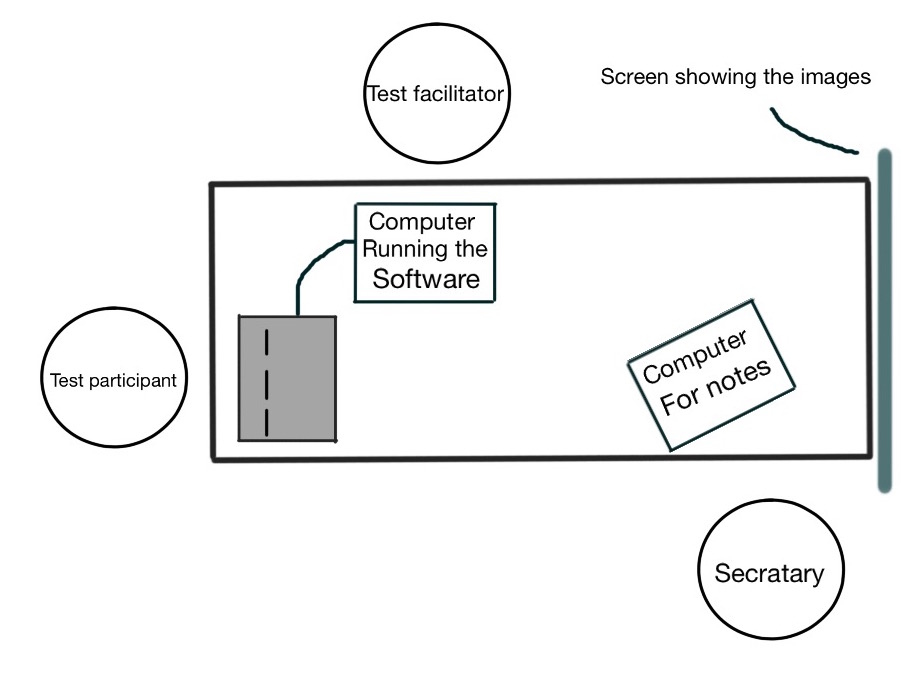
\includegraphics[width=1\textwidth]{testsetup}
\caption{\label{fig:testsetup} Illustration of the test set-up.}
\end{figure}

The final test was conducted on 15 test participants from Aalborg University in their 20's. The participants consisted of 14 students from medialogy and one student from Art \& Technology. \todo{dette kan bruges i diskution, da vi ville have faaet mere variation i resultaterne hvis vi fx. havde testet paa museumsgaester i alle aldre} The test took place in a small closed room located at Rendsburggade 14. The test was conducted by a test facilitator; who interviewed the participants and instructed which tasks to perform while observing the software during the test. During the testing a secretary would take notes of the entire test. Furthermore, the prototype was placed in front of the participants and a laptop was used to display the two pictures the project group decide to use during the test. The facilitator would change the picture on the laptop since it was not automatised and worked independently from the actual software and was only used to display the pictures.   

\begin{figure}[!h] 
\centering
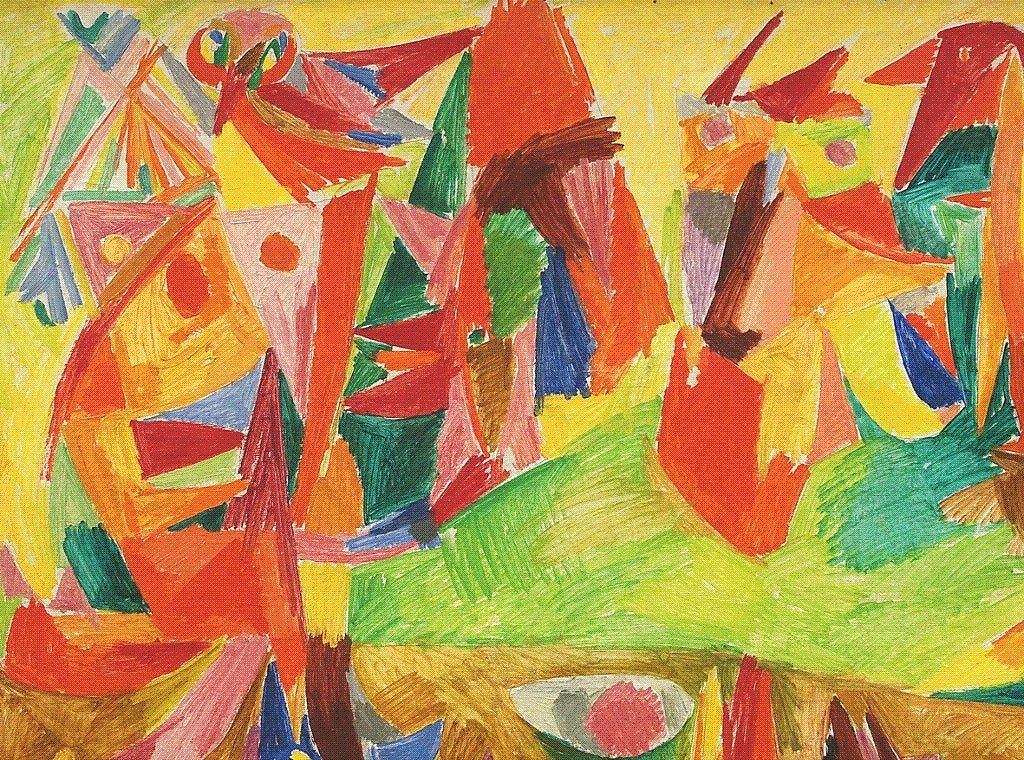
\includegraphics[width=1\textwidth]{asger}
\caption{\label{fig:asger} Asger Jorns "Trolden og Fuglene" 1944.}
\end{figure}

\begin{figure}[!h] 
\centering
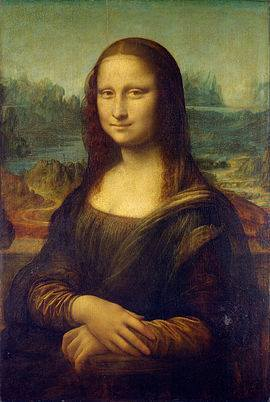
\includegraphics[width=0.5\textwidth]{monalisa}
\caption{\label{fig:monalisa} Leonardo Da Vinci "Mona Lisa" 1503-1517.}
\end{figure}

The test was carried out by welcoming the test participants in the room, one at the time. The participants were places at the end of the table and was asked to sign a consent form. The facilitator then started the test by introducing the overall project and explaining what the participant was expected to do during the test. The facilitator conducted the test by using the script shown below:


\section{Script}
The following text is the actual script, followed during the test.

Hello and thank you for wanting to participate in this test. We are group 30.

Our prototype takes an image and turns it into a sound. During this test we will give you a few different assignments and ask you questions during the test. This is a test of the product, and we prefer you to think out loud during the test.

//Mona Lisa is shown on the screen 
Questions: 


\begin{itemize}
\item What do you think you have to do with this product?
\item What happens when you manipulated with the sliders?
\item Can you hear a difference between “MIN” and “MAX”?
\item Can you hear a difference between the effects?
\item Is the “help text” helpfull to you?
\item Is the help text clear?
\item Any other thoughts?
\end{itemize}


/* Now we will change the images to Asgar Jorn */
\begin{itemize}
\item Do you hear the difference between the two pictures?
\item Why do you think there is a difference between the images?
\item Can you hear a difference between “MIN” and “MAX”?
\item Can you hear a difference between the effects?
\end{itemize}


Any other overall thoughts?

\section{Evaluation results}

Comb filter results

\begin{table}[!h]
\centering
\caption{}
\label{tab:comb}
\begin{tabular}{|l|c|c|c|c|c|c|c|c|c|c|c|c|c|c|c|c|c|}
\hline
\multicolumn{18}{|c|}{Can you hear the difference between the "MIN" and "MAX" on the Comb filter?} \\ \hline
\multicolumn{2}{|l|}{} & \multicolumn{15}{c|}{Amount of participants} & \textbf{Total} \\ \hline
\multirow{2}{*}{\begin{tabular}[c]{@{}l@{}}Mona \\ Lisa\end{tabular}} & Yes &  &  &  &  &  &  &  &  &  &  &  &  & X &  &  & \textbf{1} \\ \cline{2-18} 
 & No & X & X & X & X & X & X & X & X & X & X & X & X &  & X & X & \textbf{14} \\ \hline
\multirow{2}{*}{\begin{tabular}[c]{@{}l@{}}Asgar \\ Jorn\end{tabular}} & Yes &  &  &  &  &  &  &  &  &  &  & X &  & X &  &  & \textbf{2} \\ \cline{2-18} 
 & No & X & X & X & X & X & X & X & X & X & X &  & X &  & X & X & \textbf{13} \\ \hline
\end{tabular}
\end{table}

Bandpass Results
\begin{table}[]
\centering
\caption{}
\label{tab:bandpass}
\begin{tabular}{|l|c|c|c|c|c|c|c|c|c|c|c|c|c|c|c|c|c|}
\hline
\multicolumn{18}{|c|}{Can you hear the difference between the "MIN" and "MAX" on the Bandpass filter?} \\ \hline
\multicolumn{2}{|l|}{} & \multicolumn{15}{c|}{Amount of participants} & \textbf{Total} \\ \hline
\multirow{2}{*}{\begin{tabular}[c]{@{}l@{}}Mona \\ Lisa\end{tabular}} & Yes & X & X &  & X & X & X & X &  & X & X & X & X & X &  &  & \textbf{11} \\ \cline{2-18} 
 & No &  &  & X &  &  &  &  & X &  &  &  &  &  & X & X & \textbf{4} \\ \hline
\multirow{2}{*}{\begin{tabular}[c]{@{}l@{}}Asgar \\ Jorn\end{tabular}} & Yes & X & X & X & X & X & X & X &  & X & X & X & X & X &  & X & \textbf{13} \\ \cline{2-18} 
 & No &  &  &  &  &  &  &  & X &  &  &  &  &  & X &  & \textbf{2} \\ \hline
\end{tabular}
\end{table}


High shelf results
\begin{table}[]
\centering
\caption{}
\label{tab:highshelf}
\begin{tabular}{|l|c|c|c|c|c|c|c|c|c|c|c|c|c|c|c|c|c|}
\hline
\multicolumn{18}{|c|}{Can you hear the difference between the "MIN" and "MAX" on the High Shelf filter?} \\ \hline
\multicolumn{2}{|l|}{} & \multicolumn{15}{c|}{Amount of participants} & \textbf{Total} \\ \hline
\multirow{2}{*}{\begin{tabular}[c]{@{}l@{}}Mona \\ Lisa\end{tabular}} & Yes & X & X & X & X & X & X & X & X & X & X & X & X & X & X & X & \textbf{15} \\ \cline{2-18} 
 & No &  &  &  &  &  &  &  &  &  &  &  &  &  &  &  & \textbf{0} \\ \hline
\multirow{2}{*}{\begin{tabular}[c]{@{}l@{}}Asgar \\ Jorn\end{tabular}} & Yes & X & X & X & X & X & X & X & X & X & X & X & X & X & X & X & \textbf{15} \\ \cline{2-18} 
 & No &  &  &  &  &  &  &  &  &  &  &  &  &  &  &  & \textbf{0} \\ \hline
\end{tabular}
\end{table}

Is the "help text" useful you you?
\begin{table}[!h]
\centering
\caption{}
\label{tab:helptext}
\begin{tabular}{|l|c|c|c|c|c|c|c|c|c|c|c|c|c|c|c|c|}
\hline
\multicolumn{17}{|c|}{Is the "help text" usefull to you?} \\ \hline
 & \multicolumn{15}{c|}{Amount of participants} & \textbf{Total} \\ \hline
Yes &  & X & X & X & X & X & X & X & X & X & X & X & X & X & X & \textbf{14} \\ \hline
No & X &  &  &  &  &  &  &  &  &  &  &  &  &  &  & \textbf{1} \\ \hline
\end{tabular}
\end{table}

Can you hear a difference between the two images?
\begin{table}[!h]
\centering
\caption{}
\label{tab:twoimagedifference}
\begin{tabular}{|l|c|c|c|c|c|c|c|c|c|c|c|c|c|c|c|c|}
\hline
\multicolumn{17}{|c|}{Can you hear a difference between the two images?} \\ \hline
 & \multicolumn{15}{c|}{Amount of participants} & \textbf{Total} \\ \hline
Yes & X & X & X & X & X & X & X & X & X & X & X & X & X & X & X & \textbf{15} \\ \hline
No &  &  &  &  &  &  &  &  &  &  &  &  &  &  &  & \textbf{0} \\ \hline
\end{tabular}
\end{table}


\section{Results analysis}

This section contains the analysis of the test results. The analysis methods are outlined and then used. 

%The results were found by making a semi-structured interview and getting qualitative feedback by communicating directly with the user, using the script shown above.

For statistical analysis of quantitative data, Fisher's exact test is used to determine whether there is a connection between explanatory variables and their contingencies. This test is specifically concerned with the influence the two different images have on our results. Binomial tests are used to determine the significance of our results. An significance value $\alpha$ of 0.05 is used.

The product must be able to audiolise the image. For this criteria to be fulfilled, individual images must produce audio that is distinct. The user test shows that images produce a unique sound. This can be seen in the fact that all test participants could hear a clear difference between the colourful Asger Jorn painting and the darker Mona Lisa painting ($p=6.104e-5$). 

The effects that are applied to this audiolisation must be alterable by the user. The technical test shows that the audio filters are applied as desired - the filter responses match what is expected from the respective types of filter. There is an underlying assumption to this criteria that this effect must be discernable by the user, otherwise there is no point to it. Using Fisher's exact test it is first determined whether the image has an influence on whether the user can hear the effect. There is no significant correlation between the image used and the users ability to hear the affect for any of the filters ($p_{comb}=1$, $p_{bandpass}=0.6513$, $p_{highshelf}=1$). Then we determine whether users can hear a difference between a filter being a applied or not applied. Users determined that they could hear the bandpass filter ($p=0.001431$) and the high shelf filter ($p=1.863e-09$). They also determined they could NOT hear the comb filter ($p=8.43e-06$).

Finally the product must be usable. The interface was clear for all the participants and they knew how to use it, either by looking at the help text or at the sliders. None of the test participants had any trouble manipulating with the sliders. Nine of the participants did not know the terms of the different filters, but they could distinguish a change in the output when manipulating with the sliders. However, all users found the help text helpful. This indicates that the principle of using text labels to explain certain elements of this kind of interface is sound, but that the current implementation of this is problematic. The biggest issue here is probably that the labels make use of technical language which only provides useful information for expert users.
 
